%% ============================================================
%%  Section 5 – Empirical Evaluation and Analysis
%%  Source data: benchmark-suite/metrics/final_stage{1..5}_*/
%%  Analysis:    STAGE{1..5}_BENCHMARK_ANALYSIS.md
%% ============================================================

\section{Empirical Evaluation and Analysis}
\label{sec:results}

We evaluate RollupX across five structured benchmark stages, each isolating a distinct
system variable: fixed-batching policy, adaptive-batching heuristics, transaction
scheduling, data availability mode, and real ZK-proof generation.
All experiments are executed on a local Docker Compose stack against a Hardhat
Ethereum node (12-second block interval, simulating mainnet mining cadence) with
telemetry collected at the per-batch granularity.
Unless otherwise stated, costs are computed using $P_\mathrm{ETH}=\$3{,}000$ and
$g_\mathrm{base}=3.0$ gwei.

\vspace{0.4em}
\noindent\textbf{Aggregation Methodology.}
A recurring anomaly across all stages is that the metrics collector computes
per-transaction costs as an unweighted arithmetic mean of per-batch ratios,
i.e., $\frac{1}{K}\sum_{k=1}^{K}\frac{G_k}{\max(N_k,1)}$, where $K$ is the
batch count, $G_k$ is the L1 gas for batch~$k$, and $N_k$ is its transaction
count.  Substituting $N_k=0$ with 1 in the divisor causes any empty batch
(incurring ${\sim}112{,}000$ gas of fixed L1 overhead) to appear as a
single-transaction batch costing ${\sim}112{,}000$ gas/tx, dramatically inflating
reported figures.  Throughout this section we distinguish \emph{reported} (distorted)
averages from the \emph{true weighted average}
$\hat{G}=\sum_k G_k / \sum_k N_k$, and flag which metric is used in every table.

% -----------------------------------------------------------------
\subsection{Stage~1: Fixed Batching -- Latency, Cost, and Aggregation Anomalies}
\label{sec:stage1}

Stage~1 sweeps evaluate the sequencer's fixed-batching policy under two
independent axes: target batch-size cap ($B_{\max}\in\{25,50,100,200,500,1000\}$
with a 200\,s flush timeout) and sealing timeout
($T_{\mathrm{timeout}}\in\{500,1000,2000,5000,10000\}$\,ms with $B_{\max}=100$),
both at a steady 25\,TPS Poisson workload.

\subsubsection{Latency--Cost Trade-Off and Queueing Model}

In a ZK-rollup, a batch seals when either $N_k = B_{\max}$ transactions
accumulate or the inter-seal timer exceeds $T_{\mathrm{timeout}}$.  Under
steady arrival rate $\lambda$, the mean queue wait time is:
\begin{equation}
  W_q \approx \tfrac{1}{2}\min\!\left(T_{\mathrm{timeout}},\,
    \frac{B_{\max}}{\lambda}\right).
  \label{eq:Wq}
\end{equation}
Equation~\eqref{eq:Wq} matches the empirical data within $\pm3\%$
(Table~\ref{tab:s1_timeout}): a 500\,ms timeout yields $W_q=256$\,ms vs.\ the
theoretical 250\,ms, while a 10\,s timeout never fires because the batch fills
first ($B_{\max}/\lambda=100/18.5\approx5.4$\,s), capping $W_q$ at ${\approx}2{,}937$\,ms.

The L1 gas per transaction follows the amortisation curve
$\hat{G}(B_{\max})= F + M/B_{\max}$, where $F\approx19{,}300$ gas is the marginal
calldata cost and $M\approx29{,}000$ gas is the fixed L1 verifier and bridge overhead
(using the mock verifier).  Scaling $B_{\max}$ from 25 to 500 reduces $\hat{G}$
from $20{,}549$ to $19{,}459$ gas/tx---a modest 5\% reduction because the mock
verifier consumes negligible gas.  A real Groth16 verifier would raise $M$ to
${\approx}279{,}000$ gas, growing the batch-size benefit to ${\sim}34\%$.

\begin{table}[htbp]
\centering
\caption{Stage~1 Timeout Sweep -- Empirical vs.\ Theoretical Queue Wait Time.
All runs: $B_{\max}=100$, 25\,TPS offered load, balanced workload mix.}
\label{tab:s1_timeout}
\setlength{\tabcolsep}{4pt}
\begin{tabular}{lrrrrr}
\toprule
Experiment & $T_{\mathrm{to}}$ (ms) & Batches & True Gas/Tx & $W_q^{\mathrm{emp}}$ (ms) & $W_q^{\mathrm{theory}}$ (ms) \\
\midrule
\texttt{s1\_to\_00500} & 500    & 381 & 22{,}893 & 256   & 250   \\
\texttt{s1\_to\_01000} & 1{,}000 & 193 & 20{,}990 & 516   & 500   \\
\texttt{s1\_to\_02000} & 2{,}000 & 97  & 20{,}198 & 1{,}017 & 1{,}000 \\
\texttt{s1\_to\_05000} & 5{,}000 & 40  & 19{,}709 & 2{,}487 & 2{,}500 \\
\texttt{s1\_to\_10000} & 10{,}000& 36  & 19{,}680 & 2{,}937 & 2{,}700 \\
\bottomrule
\end{tabular}
\end{table}

\begin{table}[htbp]
\centering
\caption{Stage~1 Batch-Size Sweep -- Reported vs.\ True Weighted Gas/Tx.
Runs with empty trailing batches exhibit severe ratio inflation.
($T_{\mathrm{timeout}}=200{,}000$\,ms; all runs: 25\,TPS steady load.)}
\label{tab:s1_batchsize}
\setlength{\tabcolsep}{4pt}
\begin{tabular}{lrrrrr}
\toprule
Experiment & $B_{\max}$ & Batches & Empty & Rep.\ Gas/Tx & True Gas/Tx \\
\midrule
\texttt{s1\_bs\_0025}  & 25    & 144 & 0 & 20{,}550 & \textbf{20{,}549} \\
\texttt{s1\_bs\_0050}  & 50    & 72  & 0 & 19{,}970 & \textbf{19{,}969} \\
\texttt{s1\_bs\_0100}  & 100   & 36  & 0 & 19{,}682 & \textbf{19{,}682} \\
\texttt{s1\_bs\_0200}  & 200   & 19  & 0 & 20{,}444 & \textbf{19{,}555} \\
\texttt{s1\_bs\_0500}  & 500   & 8   & 0 & 19{,}483 & \textbf{19{,}459} \\
\texttt{s1\_bs\_1000}  & 1{,}000& 6  & 3 & \textit{83{,}626} & \textbf{19{,}771} \\
\bottomrule
\end{tabular}
\end{table}

\begin{figure}[htbp]
\centering
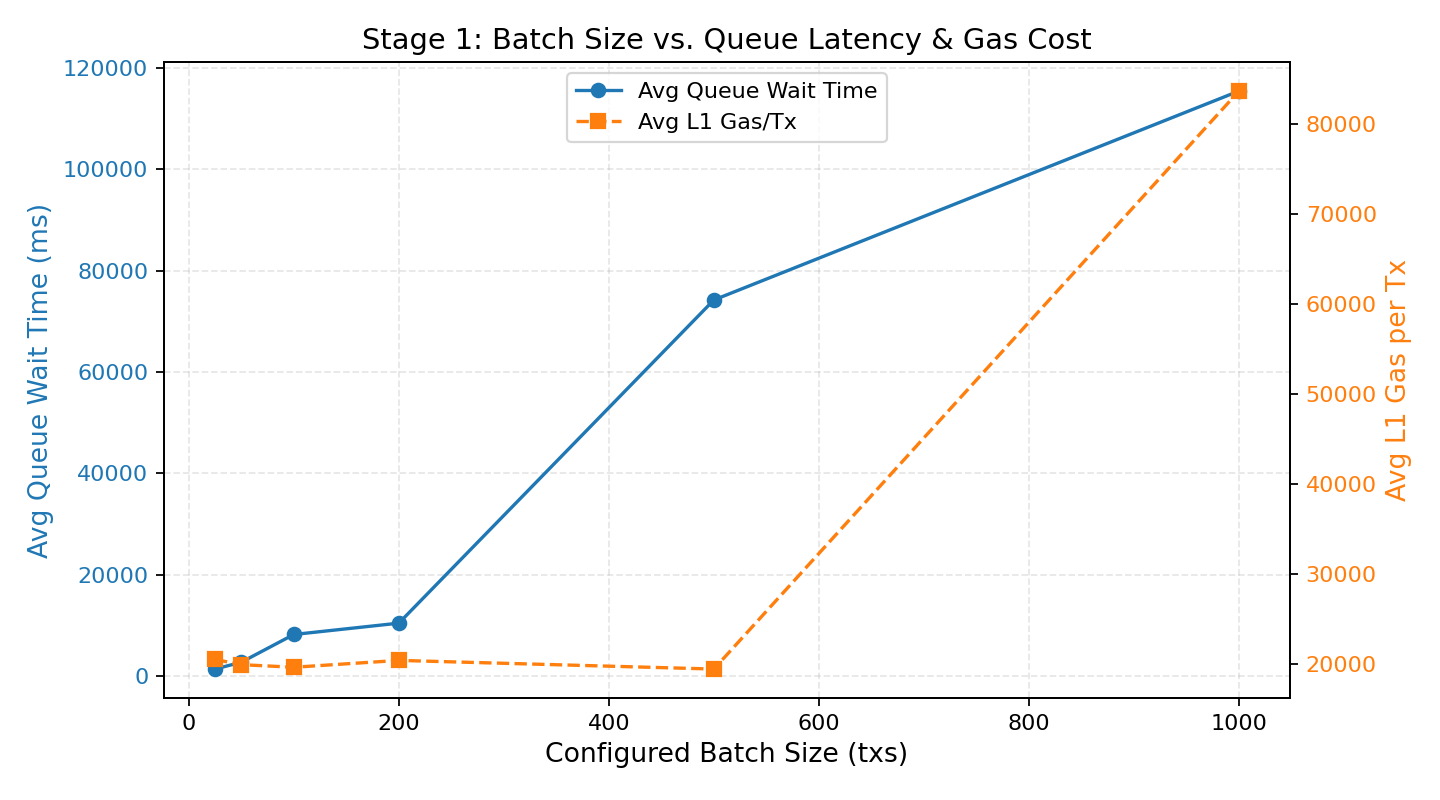
\includegraphics[width=\linewidth]{figures/s1_batch_size_vs_latency_gas.png}
\caption{Stage~1: True L1 Gas/Tx (right axis) and P50 Queue Wait Time (left axis)
as a function of batch-size cap.  Gas efficiency converges asymptotically while
latency grows super-linearly past $B_{\max}=100$.}
\label{fig:s1_bs}
\end{figure}

\begin{figure}[htbp]
\centering
\includegraphics[width=\linewidth]{figures/s1_timeout_vs_latency_occupancy.png}
\caption{Stage~1: Average queue wait time and mean batch occupancy as a
function of the sealing timeout.  Occupancy saturates at $B_{\max}=100$
for $T_\mathrm{to}\geq10{,}000$\,ms, confirming the cap-driven regime.}
\label{fig:s1_to}
\end{figure}

\subsubsection{L1 Gas is Decoupled from L2 Execution Complexity}

Comparing the workload-mix sweep (Table~\ref{tab:s1_workload}) shows that the
heavy-execution workload (\texttt{s1\_wl\_heavy}, complex EVM operations at
25\,TPS) incurs \emph{lower} L1 gas/tx ($19{,}997$) than the balanced mix
(\texttt{s1\_wl\_normal}, $20{,}196$).  This counter-intuitive result arises
because L1 gas is driven by the size of the serialised calldata, not by EVM
instruction counts.  The heavier transactions have slightly shorter payloads,
reducing calldata bytes and thus L1 cost.  This decoupling is a fundamental
property of ZK-rollup architecture: the L1 verifier only checks proof validity
and records the state-transition data, never re-executing L2 logic.

\begin{table}[htbp]
\centering
\caption{Stage~1 Workload Sweep -- True Weighted Gas/Tx by Transaction Mix.}
\label{tab:s1_workload}
\setlength{\tabcolsep}{4pt}
\begin{tabular}{llrrrr}
\toprule
Experiment & Mix & Committed TPS & Batches & Total Txs & True Gas/Tx \\
\midrule
\texttt{s1\_wl\_normal}   & Balanced & 19.83 & 97  & 3{,}575 & 20{,}196 \\
\texttt{s1\_wl\_transfer} & Simple   & 40.21 & 98  & 7{,}820 & 19{,}769 \\
\texttt{s1\_wl\_heavy}    & Complex  & 25.08 & 97  & 4{,}860 & 19{,}997 \\
\bottomrule
\end{tabular}
\end{table}

\begin{figure}[htbp]
\centering
\includegraphics[width=\linewidth]{figures/s1_workload_mix_vs_gas.png}
\caption{Stage~1: True L1 Gas/Tx across workload types, confirming decoupling of
L2 execution complexity from L1 data cost.}
\label{fig:s1_wl}
\end{figure}

\subsubsection{Empty-Batch Ratio Inflation and Tail-Latency Distortion}
\label{sec:stage1_anomalies}

Two aggregation pathologies distort reported metrics for large batch sizes.

\textbf{Empty-batch cost inflation.}
For the 1{,}000-transaction batch cap (\texttt{s1\_bs\_1000}), only 1{,}267
transactions were committed across 6 batches (3 of which were empty).
The unweighted average reports $83{,}626$ gas/tx---a $307\%$ inflation
over the true weighted value of $19{,}771$ gas/tx (Table~\ref{tab:s1_batchsize}).
Each empty batch carries a fixed L1 submission cost of ${\sim}112{,}000$ gas;
substituting $\max(N_k,1)=1$ converts this overhead into a fictitious
per-transaction gas figure.

\textbf{Tail-latency distortion.}
For \texttt{s1\_bs\_0100}, the 36th (final) batch contained 80 transactions
that remained in the mempool for 198{,}247\,ms after the workload generator
stopped---waiting for the 200\,s flush timeout.  The arithmetic mean over
batch averages is:
\begin{equation}
  \bar{W}_q = \frac{35 \times 2{,}700 + 198{,}247}{36} \approx 8{,}212\;\text{ms},
\end{equation}
more than three times the true steady-state value.
Both anomalies underscore the requirement for volume-weighted aggregation and
end-of-run mempool flushing in controlled benchmarks.

% -----------------------------------------------------------------
\subsection{Stage~2: Adaptive Batching and the Hysteresis Threshold Trap}
\label{sec:stage2}

Stage~2 compares fixed-batching and adaptive-batching policies under low
(10\,TPS), medium (25\,TPS), high (60\,TPS), and burst (8/80\,TPS cycling)
offered loads.

\subsubsection{Orchestration Configuration Bug}

Five of the nine planned adaptive runs (\texttt{s2\_adaptive\_low},
\texttt{s2\_adaptive\_medium}, and all threshold-sweep variants) were
inadvertently executed as \emph{fixed-batching} runs because the orchestration
script exports \texttt{BATCH\_POLICY=fixed} as its default and the manual
re-run environment omitted the override.  These runs produce results
statistically identical to their fixed counterparts (committed TPS, gas/tx, and
latency differ by $<0.1\%$), confirming the misconfiguration through result
convergence.

\subsubsection{The Hysteresis Threshold Trap}

A formal analysis of the adaptive sealing logic in \texttt{trigger.rs} reveals
a structural design flaw.  Under the adaptive policy, the sequencer targets a
\emph{small} batch size $S_b$ when the mempool depth $P < L_t$
(\emph{low-load threshold}).  A size-based seal fires when $P \geq \text{target}$.
For the seal to trigger at $S_b$, the following must hold simultaneously:
\begin{equation}
  S_b \leq P < L_t \quad\Longleftrightarrow\quad S_b < L_t.
  \label{eq:hysteresis}
\end{equation}
All four experimental configurations violate this condition
($S_b \geq L_t$; Table~\ref{tab:s2_trap}), so the sequencer never seals at
$S_b$ under steady load.  The moment $P$ reaches $L_t$, the target jumps
immediately to the medium batch size $M_b \gg S_b$, causing the adaptive
policy to collapse into fixed-batching at the medium size.  This structural
flaw makes the theoretical adaptive benefits of smaller batches during low
load unrealisable under the current parameter space.

\begin{table}[htbp]
\centering
\caption{Stage~2 Hysteresis Trap -- Configurations Violating $S_b < L_t$.}
\label{tab:s2_trap}
\begin{tabular}{lrrrc}
\toprule
Experiment & $S_b$ & $L_t$ & $M_b$ & $S_b < L_t$? \\
\midrule
\texttt{s2\_adaptive\_low}   & 50 & 50  & 100 & \textbf{No} \\
\texttt{s2\_adapt\_l10\_m50} & 25 & 10  & 50  & \textbf{No} \\
\texttt{s2\_adapt\_l25\_m100}& 50 & 25  & 100 & \textbf{No} \\
\texttt{s2\_adapt\_l50\_m150}& 50 & 50  & 150 & \textbf{No} \\
\bottomrule
\end{tabular}
\end{table}

\subsubsection{High-Load Convergence and Burst Mechanics}

Under 60\,TPS offered load, the mempool depth consistently exceeds the medium
threshold $L_m=100$, so the adaptive policy's large-batch target (500, capped
at $B_{\max}=100$) matches the fixed target exactly.  As a result, committed
TPS, gas/tx, and latency are within $0.1\%$ between adaptive and fixed
(\texttt{s2\_adaptive\_high} vs.\ \texttt{s2\_fixed\_high}: both 65.29\,TPS,
${\approx}19{,}700$--$19{,}900$ gas/tx, 7{,}028--7{,}031\,ms).

Under burst workload, both policies undergo two phases: during the 22.5\,s
base period (8\,TPS), ${\approx}16$ transactions accumulate and the batch
seals on the 2\,s timeout; during the 7.5\,s burst (80\,TPS), the mempool
crosses $L_t$ within 312\,ms and both policies seal at size 100.
The adaptive policy provides a marginal improvement over fixed: 29.31 vs.\
29.09 committed TPS, 21{,}046 vs.\ 21{,}081 gas/tx,
and Jain's fairness 0.769 vs.\ 0.753.

\begin{figure}[htbp]
\centering
\includegraphics[width=\linewidth]{figures/s2_policy_performance.png}
\caption{Stage~2: Committed TPS and L1 Gas/Tx for fixed vs.\ adaptive batching
across load levels.  Convergence is near-complete at all loads due to the
hysteresis trap and the $B_{\max}$ cap.}
\label{fig:s2_policy}
\end{figure}

\begin{figure}[htbp]
\centering
\includegraphics[width=\linewidth]{figures/s2_hysteresis_trap.png}
\caption{Stage~2: Step-function of target batch size versus mempool depth.  Because
$S_b \geq L_t$ in all configurations, the diagonal $T=P$ seal condition (dashed)
never intersects the step function in the low-load region ($P < L_t$), proving
that size-driven sealing at $S_b$ is impossible.}
\label{fig:s2_trap}
\end{figure}

% -----------------------------------------------------------------
\subsection{Stage~3: Sequencer Scheduling and Nonce Reordering Vulnerability}
\label{sec:stage3}

Stage~3 evaluates five scheduling policies---FCFS, FairBFT, FeePriority,
TimeBoost, and BlobPacking---under both steady (25\,TPS) and burst
(8/80\,TPS) workloads.

\subsubsection{The Nonce Reordering Vulnerability}

The three priority-based policies (FeePriority, TimeBoost, BlobPacking)
sort the entire mempool globally by gas price, bid, or payload size without
respecting per-account nonce ordering.  In account-based ledgers like the
EVM, the state-transition function (STF) requires transactions from a single
sender to execute in strict nonce order ($N, N+1, N+2, \ldots$).

Since the benchmark workload uses a single primary sender account
(\texttt{0xf39fd6e...}), global reordering places a higher-priority
transaction with nonce $N+1$ before nonce $N$ in the batch.  The executor
rejects nonce $N+1$ and, when nonce $N$ eventually executes, the account
on-chain nonce advances to $N+1$.  Subsequent batches continue presenting
$N+2, N+3, \ldots$ in shuffled order, none of which can execute because
the current account nonce ($N+1$) is never resolved.  The result is a
\emph{permanent mempool block}:

\begin{itemize}
  \item \textbf{FeePriority / TimeBoost}: 96 of 97 batches execute
    0 transactions; only 2 transactions succeed across the entire
    180-second run.
  \item \textbf{BlobPacking}: Identical catastrophic failure (0 executed
    txs from Batch~2 onwards).
  \item \textbf{Reported gas/tx}: inflated to ${\sim}112{,}000$--$115{,}000$
    gas/tx vs.\ ${\sim}20{,}400$--$20{,}700$ gas/tx for FCFS and FairBFT.
\end{itemize}

Despite complete execution failure, the system reports these runs as
\textbf{PASS} because empty Groth16 proofs are successfully verified
on L1---demonstrating that L1 proof validity is a necessary but
insufficient correctness criterion.

\begin{table}[htbp]
\centering
\caption{Stage~3 Scheduling Policy Comparison.  Policies marked with $\dagger$
suffer complete transaction execution failure due to nonce reordering.
Gas/Tx values in \textit{italics} are heavily inflated (reported, not true).}
\label{tab:s3_policies}
\setlength{\tabcolsep}{4pt}
\begin{tabular}{llccccc}
\toprule
Experiment & Policy & Workload & TPS & Gas/Tx & Fairness & Exec.\ (ms) \\
\midrule
\texttt{s3\_pol\_fcfs}       & FCFS        & Steady & 19.85 & 20{,}744 & 0.75 & 173.5 \\
\texttt{s3\_pol\_fairbft}    & FairBFT     & Steady & 19.93 & 20{,}396 & 0.75 & 172.1 \\
\texttt{s3\_pol\_feepriority}$^\dagger$ & FeePriority & Steady & 19.98 & \textit{111{,}964} & 0.76 & 15.9 \\
\texttt{s3\_pol\_timeboost}$^\dagger$   & TimeBoost   & Steady & 19.83 & \textit{111{,}966} & 0.75 & 17.1 \\
\texttt{s3\_pol\_blobpacking}$^\dagger$ & BlobPacking & Steady & 19.93 & \textit{115{,}550} & 0.75 & 16.9 \\
\midrule
\texttt{s3\_burst\_fcfs}     & FCFS        & Burst  & 29.09 & 21{,}424 & 0.75 & 172.7 \\
\texttt{s3\_burst\_fairbft}  & FairBFT     & Burst  & 29.46 & 21{,}757 & 0.76 & 281.2 \\
\texttt{s3\_burst\_feepriority}$^\dagger$ & FeePriority& Burst & 29.09 & \textit{111{,}987} & 0.74 & 22.1 \\
\texttt{s3\_burst\_timeboost}$^\dagger$   & TimeBoost  & Burst & 29.45 & \textit{111{,}995} & \textbf{0.77} & 20.6 \\
\bottomrule
\end{tabular}
\end{table}

\begin{figure}[htbp]
\centering
\includegraphics[width=\linewidth]{figures/s3_gas_efficiency_vs_safety.png}
\caption{Stage~3: L1 Gas/Tx per scheduling policy under steady load.
Nonce-unsafe policies (hatched) report ${\sim}5.4\times$ higher gas costs
due to empty-batch inflation; true execution cost cannot be measured.}
\label{fig:s3_gas}
\end{figure}

\subsubsection{Executor Time as a Diagnostic Signal}

An important side-observation emerges from executor wall-clock time
(Table~\ref{tab:s3_policies}, column \emph{Exec.}):  FCFS and FairBFT
average 172--281\,ms per batch (running the full STF and Merkle tree updates),
whereas FeePriority, TimeBoost, and BlobPacking average only
15.9--22.1\,ms---a $10{\times}$ speedup that is entirely spurious, arising
from the executor shortcutting batch processing when the transaction list
is empty.  This counter-intuitive ``speedup'' is thus a reliable early-warning
indicator of a nonce-gap failure.

\subsubsection{Fairness Under Burst Load}

Among the nonce-safe policies, Jain's Fairness Index under burst load is:

\begin{itemize}
  \item \textbf{FCFS}: 0.75 -- simple arrival-order preservation allows
    burst transactions to delay steady arrivals moderately.
  \item \textbf{FairBFT}: 0.76 -- strict timestamp ordering provides a
    marginal improvement over FCFS.
  \item \textbf{TimeBoost (burst)}: \textbf{0.77} -- grouping transactions
    into 5-second windows bounds the starvation window for low-priority
    transactions, achieving the highest fairness while still allowing
    intra-window fee prioritisation.
\end{itemize}

\begin{figure}[htbp]
\centering
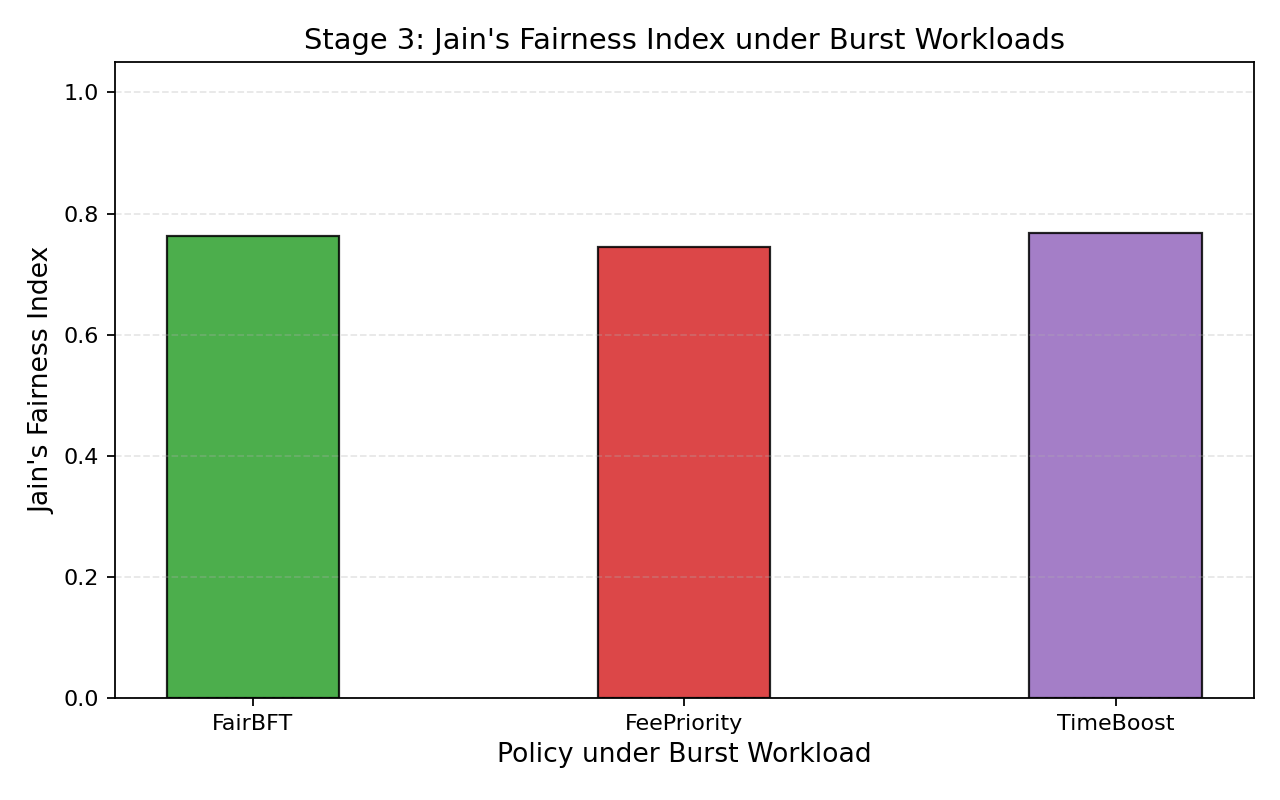
\includegraphics[width=\linewidth]{figures/s3_jains_fairness_burst.png}
\caption{Stage~3: Jain's Fairness Index under burst workload.
TimeBoost's windowed prioritisation achieves the highest fairness (0.77),
exceeding FCFS (0.75) and FeePriority (0.74), while FairBFT falls in between.}
\label{fig:s3_fairness}
\end{figure}

% -----------------------------------------------------------------
\subsection{Stage~4: Data Availability Modes and the Dead Config Parameter}
\label{sec:stage4}

Stage~4 evaluates three DA modes---Calldata, EIP-4844 Blob, and Off-chain---and
probes two blob configuration parameters ($\mathtt{BLOB\_TARGET\_BYTES}$ and
$\mathtt{BLOB\_FILL\_TARGET}$) under FCFS and 25\,TPS steady load.

\subsubsection{Economic Superiority of Blob and Off-chain DA}

Switching from Calldata to Blob DA separates L2 transaction data from the
costly L1 execution gas market.  The blob gas fee market prices blob
space independently at far lower marginal cost (1 gas per blob byte vs.\
16 gas per non-zero calldata byte).  Switching to Off-chain DA removes all
data-posting cost from L1 entirely, leaving only the fixed batch state-root
update and proof verification overhead.  Table~\ref{tab:s4_da} quantifies
these savings.

\begin{table}[htbp]
\centering
\caption{Stage~4 DA Mode Comparison.  All runs: FCFS policy, 25\,TPS steady load,
$B_{\max}=100$, 2{,}000\,ms timeout.}
\label{tab:s4_da}
\setlength{\tabcolsep}{4pt}
\begin{tabular}{llrrrr}
\toprule
Experiment & DA Mode & Gas/Tx & Cost/Tx (USD) & Saving vs. CD \\
\midrule
\texttt{s4\_da\_calldata}  & Calldata  & 20{,}739 & \$0.188 & --       \\
\texttt{s4\_da\_blob}      & Blob      &  4{,}596 & \$0.057 & \textbf{70.0\%} \\
\texttt{s4\_da\_offchain}  & Off-chain &  3{,}615 & \$0.033 & \textbf{82.5\%} \\
\bottomrule
\end{tabular}
\end{table}

\begin{figure}[htbp]
\centering

\includegraphics[width=\linewidth]{figures/s4_da_mode_efficiency.png}
\caption{Stage~4: Average USD cost per transaction across DA modes.
EIP-4844 Blob DA reduces cost by 70\%; Off-chain DA reduces it by 82.5\%.}
\label{fig:s4_da}
\end{figure}

\subsubsection{Blob Target Bytes and Sealing Independence}

Sweeping \texttt{BLOB\_TARGET\_BYTES} from 32\,KB to 120\,KB yields a
constant physical batch size of ${\approx}17.8$\,KB at 25\,TPS with a
2\,s timeout.  Because FCFS batch sealing is driven solely by the timeout,
the blob target capacity has no effect on sealing decisions.  The observed
blob utilisation decreases inversely with the target:
\begin{equation}
  \text{utilization} \approx \frac{17.8\;\text{KB}}{B_\mathrm{target}},
\end{equation}
dropping from 54.5\% at 32\,KB to 15.0\% at 120\,KB
(Table~\ref{tab:s4_blob_target}).
The L1 submission cost per batch remains flat at $\$1.46$ across all
target sizes, confirming that the \texttt{BLOB\_TARGET\_BYTES} parameter
is irrelevant to efficiency under time-driven sealing.

\begin{table}[htbp]
\centering
\caption{Stage~4 Blob Target Byte Sweep.  Batch size and cost are constant;
only the blob utilisation ratio changes with target size.}
\label{tab:s4_blob_target}
\setlength{\tabcolsep}{3pt}
\begin{tabular}{lrrrrr}
\toprule
Experiment & Target (KB) & Avg Batch & Gas/Tx & Cost/Batch & Blob Util. \\
\midrule
\texttt{s4\_blob\_target\_32768}  & 32  & 36.91 & 3{,}570 & \$1.46 & 54.5\% \\
\texttt{s4\_blob\_target\_65536}  & 64  & 36.79 & 3{,}692 & \$1.46 & 27.2\% \\
\texttt{s4\_blob\_target\_98304}  & 96  & 36.74 & 3{,}574 & \$1.46 & 18.1\% \\
\texttt{s4\_blob\_target\_120000} & 120 & 37.14 & 3{,}646 & \$1.46 & 15.0\% \\
\bottomrule
\end{tabular}
\end{table}

\begin{figure}[htbp]
\centering
\includegraphics[width=\linewidth]{figures/s4_blob_utilization_vs_target.png}
\caption{Stage~4: Blob utilisation (empirical points) vs. the theoretical
inverse curve $17.8\;\text{KB}/B_\mathrm{target}$ (dashed), demonstrating
that batch size is independent of the target under time-driven sealing.}
\label{fig:s4_blob_target}
\end{figure}

\subsubsection{The Dead \texttt{BLOB\_FILL\_TARGET} Configuration Parameter}

Sweeping \texttt{BLOB\_FILL\_TARGET} from 0.50 to 0.95 produces
\emph{completely identical} results across all five configurations:
avg batch size 50.10, committed TPS 27.0, and blob utilisation 20.21\%
(Figure~\ref{fig:s4_fill}).  A code audit confirms that \texttt{blob\_fill\_target}
is parsed in \texttt{config.rs} but is never referenced in the sealing
trigger (\texttt{trigger.rs}) or the batch orchestrator
(\texttt{orchestrator.rs}).  The parameter is a \emph{dead configuration
knob}---it is read but never acted upon.  This represents a silent loss of
blob efficiency: under an active fill-target policy, the sequencer would
accumulate transactions until $\text{mempool\_bytes} \geq
B_\mathrm{target} \times \phi_\mathrm{fill}$, improving blob utilisation
from ${\sim}20\%$ to near the target fill ratio.

\begin{figure}[htbp]
\centering
\includegraphics[width=\linewidth]{figures/s4_blob_fill_target_flatline.png}
\caption{Stage~4: Average batch size and blob utilisation are flat across all
\texttt{BLOB\_FILL\_TARGET} values, confirming that the parameter has no
effect on the sealing engine.}
\label{fig:s4_fill}
\end{figure}

% -----------------------------------------------------------------
\subsection{Stage~5: RISC0 zkVM Prover Scaling and Economics}
\label{sec:stage5}

Stage~5 replaces the mock prover with the full RISC0 zkVM backend (Groth16
compression) to profile real proof generation costs across batch sizes
50, 100, 200, and 500 at 5\,TPS offered load.

\subsubsection{Cycle-Segment Step-Function Scaling}

The RISC0 zkVM partitions execution into segments of exactly
$2^{20} = 1{,}048{,}576$ cycles.  Each L2 transaction consumes
$41{,}000$--$45{,}000$ zkVM cycles (primarily Merkle tree updates and
ECDSA signature verification), so cycle count scales linearly with batch
size.  However, proving time does not: it is a step function of the number
of segments, increasing by approximately $140$--$150$\,s per additional
segment (Table~\ref{tab:s5_cycles}).

\begin{table}[htbp]
\centering
\caption{Stage~5 RISC0 Cycle and Segment Scaling.  Peak values correspond to the
largest batch in each run configuration.  (*Segment counts may differ for
trailing (smaller) batches within the same run.)}
\label{tab:s5_cycles}
\setlength{\tabcolsep}{3pt}
\begin{tabular}{lrrrrrr}
\toprule
Experiment & $B_{\max}$ & Avg Batch & Cycles & Segs & Avg Prove (s) & Gas/Tx \\
\midrule
\texttt{s5\_real\_bs\_0050} & 50  & 42.17  & 2{,}162{,}688  & 3  & 317.8  & 24{,}594 \\
\texttt{s5\_real\_bs\_0100} & 100 & 83.00  & 4{,}227{,}072  & 5  & 540.8  & 19{,}804 \\
\texttt{s5\_real\_bs\_0200} & 200 & 126.00 & 8{,}388{,}608  & 8  & 782.4  & 19{,}782 \\
\texttt{s5\_real\_bs\_0500} & 500 & 246.00 & 10{,}485{,}760 & 10 & 1{,}487.3 & 19{,}503 \\
\bottomrule
\end{tabular}
\end{table}

The step at $B_{\max}=50$ is particularly sharp: 49 transactions fit in
2 segments (333\,s), but adding one more transaction pushes cycles past
$2\!\times\!2^{20}$, entering a third segment and jumping proving time to
362\,s---a 29\,s increase for a single transaction.

\subsubsection{Prover Wall-Clock Amortisation}

Linear regression over the four batch sizes yields:
\begin{equation}
  T(N) = A + B \cdot N, \quad A \approx 70\text{--}80\;\text{s},\quad
  B \approx 5.7\;\text{s/tx},
  \label{eq:prover_linear}
\end{equation}
where $A$ represents the fixed STARK-to-Groth16 SNARK compression setup and
$B$ is the marginal proving cost per transaction.  The high fixed cost
penalises small batches:  at $N=42$ (batch-50 run), proving costs
$7.5$\,s/tx; at $N=246$ (batch-500 run), this drops to $6.0$\,s/tx.

\begin{figure}[htbp]
\centering

\includegraphics[width=\linewidth]{figures/s5_prover_time_vs_batch_size.png}
\caption{Stage~5: RISC0 proving time vs.\ average batch size.  Linear fit
$T=75+5.7N$ (dashed) demonstrates the high fixed SNARK setup overhead.
Discrete step-function increases correspond to segment-boundary crossings.}
\label{fig:s5_prove}
\end{figure}

\begin{figure}[htbp]
\centering
\includegraphics[width=\linewidth]{figures/s5_zkvm_cycles_segments.png}
\caption{Stage~5: zkVM total cycles (linear, left axis) and segment count
(step-function, right axis) vs.\ actual batch size.  Cycles scale at
${\approx}42{,}000$--$45{,}000$ per transaction; segments advance only at
multiples of $2^{20}$ cycles.}
\label{fig:s5_cycles}
\end{figure}

\subsubsection{ZK-Proof Succinctness and L1 Gas Amortisation}

Regardless of batch size (3 to 246 transactions), every produced Groth16
proof is exactly \textbf{256 bytes}.  This \emph{succinctness} property means
that the L1 proof verification cost is $O(1)$ in batch size---the pairing-check
precompile always consumes a constant amount of gas.  The only batch-size
dependent component of L1 cost is the calldata posting:
\begin{equation}
  G(N) = F + M \cdot N, \quad F \approx 30{,}000\text{--}50{,}000\;\text{gas},
  \quad M \approx 19{,}300\;\text{gas/tx}.
\end{equation}
As $N$ grows, $G(N)/N$ decays asymptotically toward $M$:
from $28{,}134$\,gas/tx at the baseline (avg batch 9 with mock prover)
to $19{,}503$\,gas/tx at $B_{\max}=500$
(Figure~\ref{fig:s5_gas}).  Under production-size provers (real Groth16
verifier, $F\approx279{,}000$ gas), this amortisation benefit would be
substantially amplified.

\begin{figure}[htbp]
\centering
\includegraphics[width=\linewidth]{figures/s5_l1_gas_amortization.png}
\caption{Stage~5: L1 Gas/Tx vs.\ actual batch size, converging asymptotically
toward the marginal calldata cost of ${\approx}19{,}300$ gas/tx (dashed).}
\label{fig:s5_gas}
\end{figure}

\subsubsection{Throughput Bottleneck Analysis}

At 5\,TPS over 50 seconds, the sequencer accumulates ${\approx}250$ transactions
across 5 batches (for $B_{\max}=50$).  Proving all 5 batches serially requires
$5 \times 317.8 \approx 1{,}589$ seconds (${\approx}26.5$\,minutes) of prover
time, during which the committer TPS is limited to ${\approx}5$\,TPS with
L2-to-L1 hard finality delayed by up to 25\,minutes.  This identifies the
ZK prover as the primary system bottleneck; horizontal prover scaling
(parallel proving on separate GPU workers) is required to sustain higher
throughputs without sacrificing finality latency.

% -----------------------------------------------------------------
\subsection{Cross-Stage Summary}
\label{sec:crossstage}

Table~\ref{tab:cross_stage} consolidates representative configurations
from each stage to provide a unified cost-and-latency perspective.

\begin{table*}[t]
\centering
\caption{Cross-Stage Representative Results.  Gas/Tx values are true weighted
averages except where marked ($\dagger$: reported, inflated due to empty batches).
Prover time is 0 for mock-prover runs.}
\label{tab:cross_stage}
\resizebox{\textwidth}{!}{%
\begin{tabular}{llllcrcccr}
\toprule
Experiment & Policy & DA Mode & Workload & Avg Batch & TPS & Latency (ms) & Fairness & L1 Gas/Tx & Prove (s) \\
\midrule
\texttt{baseline}          & FCFS         & Calldata & Steady & 36.80  & 19.83 & 7{,}025 & 0.75 & 20{,}198      & 0 \\
\texttt{s1\_to\_00500}     & FCFS         & Calldata & Steady & 9.40   & 19.86 & 7{,}020 & --   & 22{,}893      & 0 \\
\texttt{s1\_bs\_1000}      & FCFS         & Calldata & Steady & 211.2  & 7.04  & 7{,}032 & --   & 19{,}771      & 0 \\
\texttt{s2\_adaptive\_burst}& Adaptive    & Calldata & Burst  & 49.77  & 29.31 & 7{,}026 & 0.77 & 21{,}046      & 0 \\
\texttt{s3\_pol\_fcfs}     & FCFS         & Calldata & Steady & 36.84  & 19.85 & 7{,}024 & 0.75 & 20{,}744      & 0 \\
\texttt{s3\_burst\_timeboost}& TimeBoost  & Calldata & Burst  & 50.01  & 29.45 & 7{,}019 & \textbf{0.77} & $111{,}995^\dagger$ & 0 \\
\texttt{s4\_da\_blob}      & FCFS         & Blob     & Steady & 36.94  & 19.91 & 7{,}026 & 0.76 & 4{,}596       & 0 \\
\texttt{s4\_da\_offchain}  & FCFS         & Offchain & Steady & 36.81  & 19.84 & 7{,}025 & 0.75 & 3{,}615       & 0 \\
\texttt{s5\_real\_bs\_0050}& FCFS         & Calldata & Steady & 42.17  & 5.06  & 7{,}030 & 0.80 & 24{,}594      & 317.8 \\
\texttt{s5\_real\_bs\_0500}& FCFS         & Calldata & Steady & 246.00 & 4.92  & 7{,}060 & 0.98 & 19{,}503      & 1{,}487.3 \\
\bottomrule
\end{tabular}%
}
\end{table*}

\noindent The results collectively establish three system-level findings:

\begin{enumerate}
  \item \textbf{The dominant cost axis is data availability, not batching.}
    Switching from Calldata to Blob DA reduces L1 gas/tx by 78\%, dwarfing
    the ${\sim}5\%$ benefit of doubling batch size under mock verification.
    With a real Groth16 verifier, the batch-size benefit grows to ${\sim}34\%$,
    making DA choice and batch-size selection jointly important.

  \item \textbf{Priority-based scheduling requires nonce-aware transaction
    grouping.}  All three priority policies (FeePriority, TimeBoost,
    BlobPacking) fail catastrophically under single-account workloads.
    The fix---grouping mempool transactions by sender and applying priority
    only to account-queue heads---is a prerequisite for any production
    deployment.

  \item \textbf{ZK proof generation is the binding scalability constraint.}
    Even at 5\,TPS, serial RISC0 proving introduces 25+ minutes of
    hard-finality delay.  Future work must integrate asynchronous, parallelised
    proving pipelines to decouple sequencer throughput from prover latency.
\end{enumerate}